\chapter{Introduction to Robust Control}

Robustness defines how well a system will perform in presence of:
\begin{itemize}
	\item Measurement noise: The noise in the system has to be filtered out. This in general needs to be implemented in the control system itself and the control action has to be free from the noises coming from the measurements.
	\item Disturbances: The control system should work robustly even when the disturbances to the system are random and irregular.
	\item Model Uncertainty: The control should continue to perform the required action even if there are changes in the system parameters or the system parameters were not correctly defined during the control design. Change in system parameters during operation would include for example a breakage of a rotor blade of a quad-copter.
	\item Time delays: There are time delays from the signals coming from the sensors to the control, such time delays should also not effect the quality of the control action.
\end{itemize}

In general, most of the listed characteristic required for implementing a robust control are inter-linked to each other and therefore, one characteristic cannot be improved by reducing another characteristic. For example it is not possible to improve both the noise reduction and effect of disturbances in terms of the control action. Therefore, a trade-off between various characteristics of robustness is always present.

\section{Robustness in a MIMO system}

Consider a MIMO system as shown in figure \ref{Fig_RC_MIMOsys}.
\begin{figure}[h!]
	\centering
	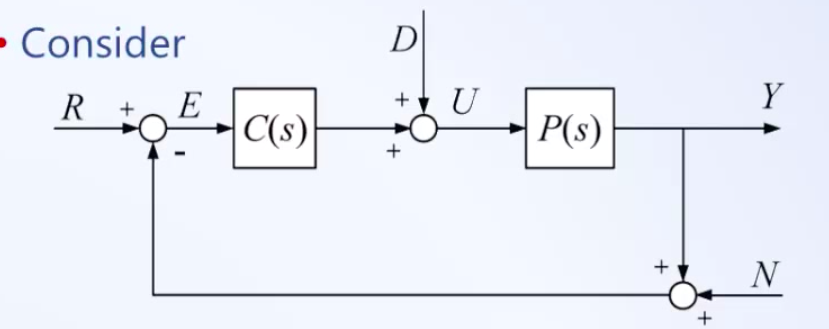
\includegraphics[width=0.8\linewidth]{Bilder/RC_MIMOsys}
	\caption{MIMO system with noise and disturbance}
	\label{Fig_RC_MIMOsys}
\end{figure}

The multiple inputs to the system are the following:
\begin{itemize}
	\item Reference $R(s)$
	\item Disturbance $D(s)$
	\item Noise $N(s)$
\end{itemize}

The effect on the system with each of these inputs can be determined by writing the TF (output/input) of the system with each of these signals as the input. For input with $R(s)$, the TF can be expressed as:
\begin{equation} \label{Eq_RC_Gyr}
	G_{yr} = \frac{Y(s)}{R(s)} = \frac{C(s)P(s)}{1 + C(s)P(s)}
\end{equation}
For the input with $D(s)$, the following TF can be expressed:
\begin{equation} \label{Eq_RC_Gyd}
	G_{yd} = \frac{Y(s)}{D(s)} = \frac{P(s)}{1 - (-P(s)C(s))} = \frac{P(s)}{1 + P(s)C(s)}
\end{equation}
with input $N(s)$, the TF can be expressed as the following:
\begin{equation} \label{Eq_RC_Gyn}
	G_{yn} = \frac{Y(s)}{N(s)} = \frac{-C(s)P(s)}{1 - (-C(s)P(s))} = \frac{-C(s)P(s)}{1 + C(s)P(s)}
\end{equation}

It can be seen that TF's $G_{yr} = - G_{yn}$, there is a direct relationship between the TF's with inputs $R(s)$ and $N(s)$. As magnitude attenuation is generally controlled using the control gain $K$, changing $K$ to attenuate $G_{yn}$ will also attenuate $G_{yr}$. Additionally, it can also be proved that 
$$ G_{yr} = - G_{yn} = \frac{P(s) - G_{yd}(s)}{P(s)} $$ Therefore, all the TF's have a relationship with each other, so changing the system gain $K$ will effect the changes in all these TF's. This relationship between all the TF's indicate that a trade-off between all these TF's have to be implemented depending on the robustness requirements.

\subsection{Attempting a control design}

\textbf{Attempt 1: }$C \rightarrow \infty$

When the control gain $K$ is increased thereby increasing the control effort $C(s)$, the following effects can be seen by each of the inputs. From equation \eqref{Eq_RC_Gyd}, the disturbance will go to zeros as the denominator of equation \eqref{Eq_RC_Gyd} will be a large number and Nr. will be a small number. On the other hand equation \eqref{Eq_RC_Gyn} for the noise will tend to $-1$. This will cause the noise amplitude to be fully transferred to the system by shifting the phase as well. So $C \rightarrow \infty$ will not solve the problem.

\textbf{Attempt 2: }$C \rightarrow 0$

From equation \eqref{Eq_RC_Gyd}, $G_{yd} \rightarrow P$. This means that the CL system will act for the disturbance in the same way as a plant would react to the signal of same input frequency. Also, from equation \eqref{Eq_RC_Gyn}, $G_{yn} \rightarrow 0$ (zero divided by any number is zero). 

From both these cases, it can be seen that either by attenuating noise or the disturbance, the other quantity gets transferred into the system. So both these quantities are dependent and they cannot be attenuated independently from the system.

\subsection{One solution from frequency response}

There is one solution to this problem of dependencies. From FrRe it can be seen that the system behaves differently for different input $\omega$. Also, based on the knowledge of input signals $D(s)$ and $N(s)$, it is seen that $N(s)$ mostly appear in high frequency input and $D(s)$ as low frequency inputs to the system. Additionally, using the knowledge of attenuation of each $D(s)$ and $N(s)$ as described in the previous section, it can be seen that $D(s)$ attenuates for larger $C(s)$ and $N(s)$ attenuates for lower $C(s)$. The control strategy considering these two parameters (high gain at low $\omega$ and vice-versa), can be laid as shown in the following figure \ref{Fig_RC_ControlStr}.
\begin{figure}[h!]
	\centering
	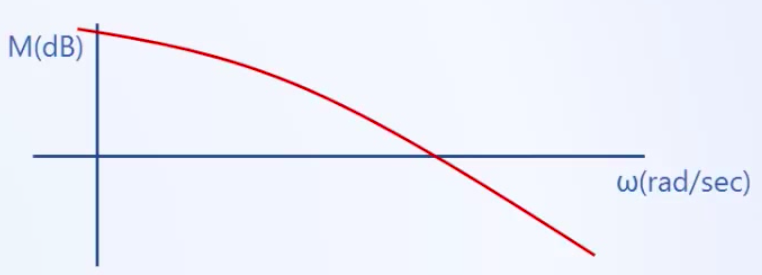
\includegraphics[width=0.8\linewidth]{Bilder/RC_ControlStr}
	\caption{Control strategy for noise and disturbance attenuation}
	\label{Fig_RC_ControlStr}
\end{figure}

Also noting that this kind of control strategy is always desirable. As the system tends to be most uncertain at higher $\omega$. Most of the time it is also difficult to record the phase change at higher $\omega$ among other model uncertainties. Attenuation would be the best possible control strategy at such regions of uncertainties.

\section{Pure Time Delay (Transport Lag)}

Another aspect in Robustness apart from Disturbance rejection and Noise canceling is to cope-up with the time-delays. Time delays are inherent in real systems. Systems such as sensors and actuators will have time delays due to the following reasons:
\begin{itemize}
	\item Discrete Sampling: The signal is read only at the end of the sampling time, so the signal would be old by the sampling time when the controller reads it.
	\item Computation time: Some of the computations would be time consuming and the controller would be reading the old computed values by the time the computation is completed.
	\item Network Delays: Most common time delays in automotive applications especially in a CAN bus. Due to this the controller would be reading old values.
\end{itemize}

\begin{figure}[h!]
	\centering
	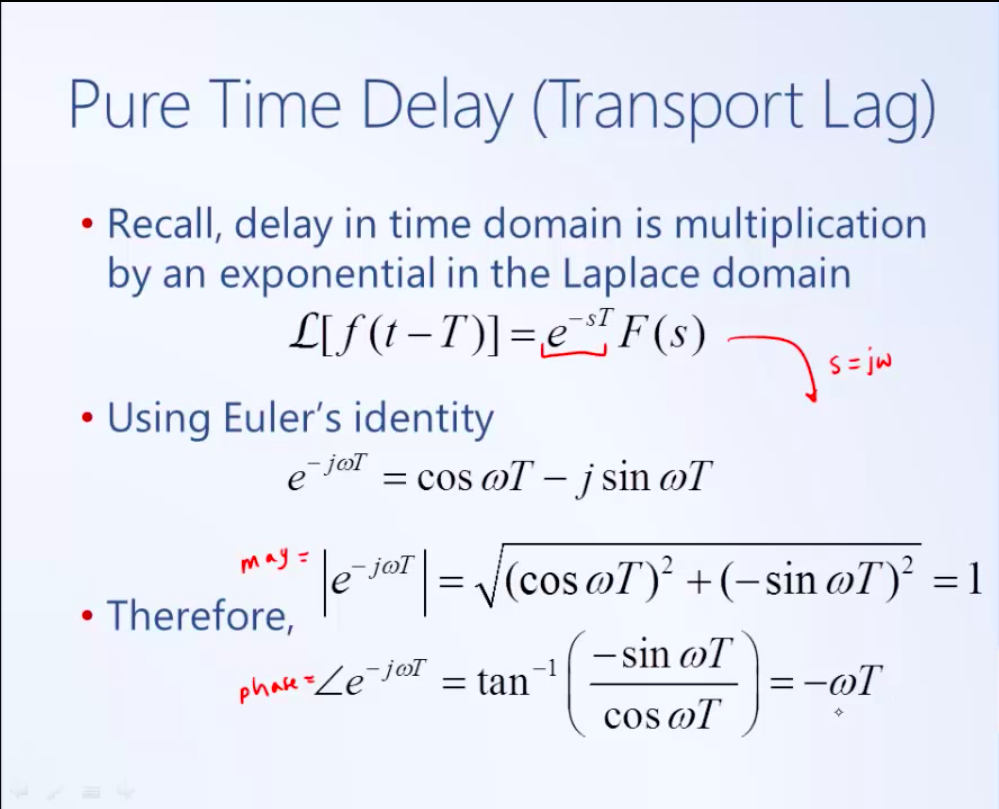
\includegraphics[width=0.8\linewidth]{Bilder/RC_TimeDelay_1}
	\caption{Time Delay theory 1}
	\label{Fig_RC_TD_1}
\end{figure}

From figure \ref{Fig_RC_TD_1}, it can be seen that the magnitude of the time delay $T$ is always $1$, a unit magnitude. However, its only the phase that changes w.r.t to the frequency of the input signal $\omega$ and the frequency lags as $\omega$ increases as $\phi = -\omega T$. Therefore, in Bode plot, time-delay can be added as a block with magnitude of $1$ and $\phi = -\omega T$.

Adding the magnitude and phase due to time-delay on the Bode plot, the new characteristic of the system can be determined. (Consider figure \ref{Fig_RC_TD_2}) This is done simply by adding the Bode plots of the system without delay (Blue line) and with delay. The red line is the result of adding Bode plot of the system without delay and with delay. The time delay with a constant magnitude $20 log 1 = 0 dB$ and phase that varies as per $\phi = -\omega T$ (converted to degrees, $T$ is time-delay in $s$) are plotted in the OL TF of the Bode plot as $$ OL = T(s)P(s) $$ $$ \angle OL = \angle T(s) + \angle P(s) $$, where $T(s)$ is the block (TF) like a control block $C(s)$ which is connected in series to the plant $P(s)$. The result is as shown in figure \ref{Fig_RC_TD_2}.

\begin{figure}[h!]
	\centering
	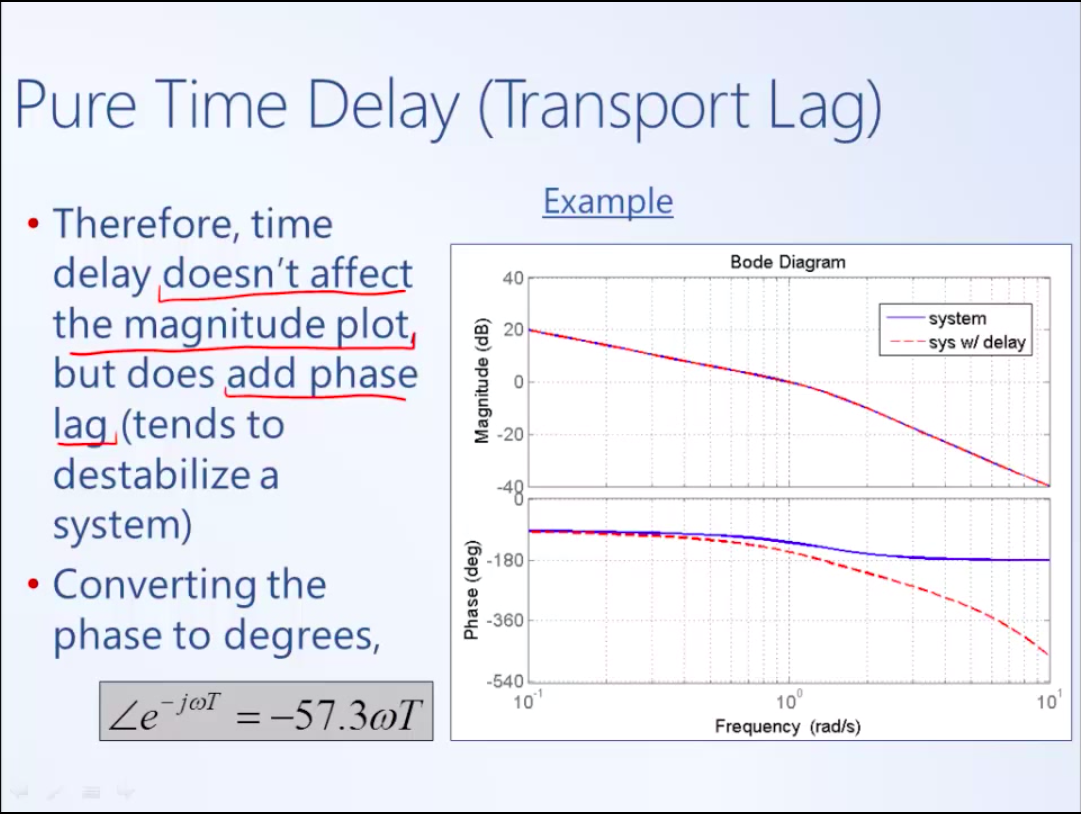
\includegraphics[width=\linewidth]{Bilder/RC_TimeDelay_2}
	\caption{Time Delay theory 2}
	\label{Fig_RC_TD_2}
\end{figure}